
\documentclass[12pt]{amsart}
\usepackage{geometry} % see geometry.pdf on how to lay out the page. There's lots.
\geometry{a4paper} % or letter or a5paper or ... etc
% \geometry{landscape} % rotated page geometry
\usepackage{graphicx} %插入图片的宏包
\usepackage{float} %设置图片浮动位置的宏包
\usepackage{subfigure} %插入多图时用子图显示的宏包
% See the ``Article customise'' template for come common customisations

\title{}
\author{}
\date{} % delete this line to display the current date

%%% BEGIN DOCUMENT
\begin{document}
\begin{figure}[H] %H为当前位置,!htb为忽略美学标准,htbp为浮动图形
\centering %图片居中
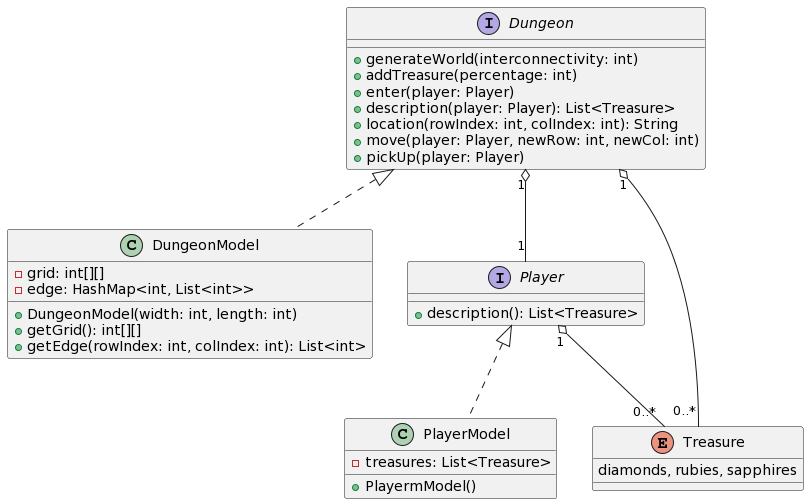
\includegraphics[width=1\textwidth]{uml.png} %插入图片,[]中设置图片大小,{}中是图片文件名
\end{figure}

\newpage

\section{Dungeon}

\begin{table}[htbp]
   %\topcaption{Table captions are better up top} % requires the topcapt package
   \begin{tabular}{@{} lll @{}} % Column formatting, @{} suppresses leading/trailing space

      Method     & Input & Expected \\
         Constructor   & Non positive width or length     &  IllegalArgumentException \\
         Constructor   & positive width and length     &  A grid of width and length and an\\ & & empty edge map\\
         generateWorld & negative interconnectivity & IllegalArgumentException\\
         generateWorld & non negative interconnectivity & Modify grid to cave and tunnel,\\& & edge to reflect connectivity between  \\ & &grids, add start and end\\
         addTreasure & negative percentage & IllegalArgumentException\\
         addTreasure &  percentage larger than 100 & IllegalArgumentException\\
         addTreasure &  valid percentage & Add Treasure to caves in grid\\
         enter & A player & Add a player to start\\
         description & A player who is not in the dungeon & IllegalArgumentException\\
         description & A player who is in the dungeon & List of Treasure\\
         location & row or column out of range & IllegalArgumentException\\
        location & valid row and column & The Treasure in this grid and \\
         && other grids it connects to\\
         move & A grid that cannot be reached in one & IllegalArgumentException\\
          & move from the current location & \\
         move & Valid grid & Change location of player\\
         pickUp & A player who is not in the dungeon & IllegalArgumentException\\
         pickUp & A player who is in the dungeon & Add Treasure to player's list\\
         getGrid & None & The grid of caves and tunnels\\
         getEdge & row and column index of the grid & Other grids that are connected \\&&to this grid\\
         
    \end{tabular}
\end{table}

%\newpage

\section{Player}
% Requires the booktabs if the memoir class is not being used

\begin{table}[htbp]
   %\topcaption{Table captions are better up top} % requires the topcapt package
   \begin{tabular}{@{} lll @{}} % Column formatting, @{} suppresses leading/trailing space

      Method      & Input & Expected \\
         Constructor        & None    &  Create a player with list of Treasure\\
         Description & None & Return the list of Treasure the player has\\

    \end{tabular}
\end{table}

\section{Final Design}
\begin{figure}[H] %H为当前位置,!htb为忽略美学标准,htbp为浮动图形
\centering %图片居中
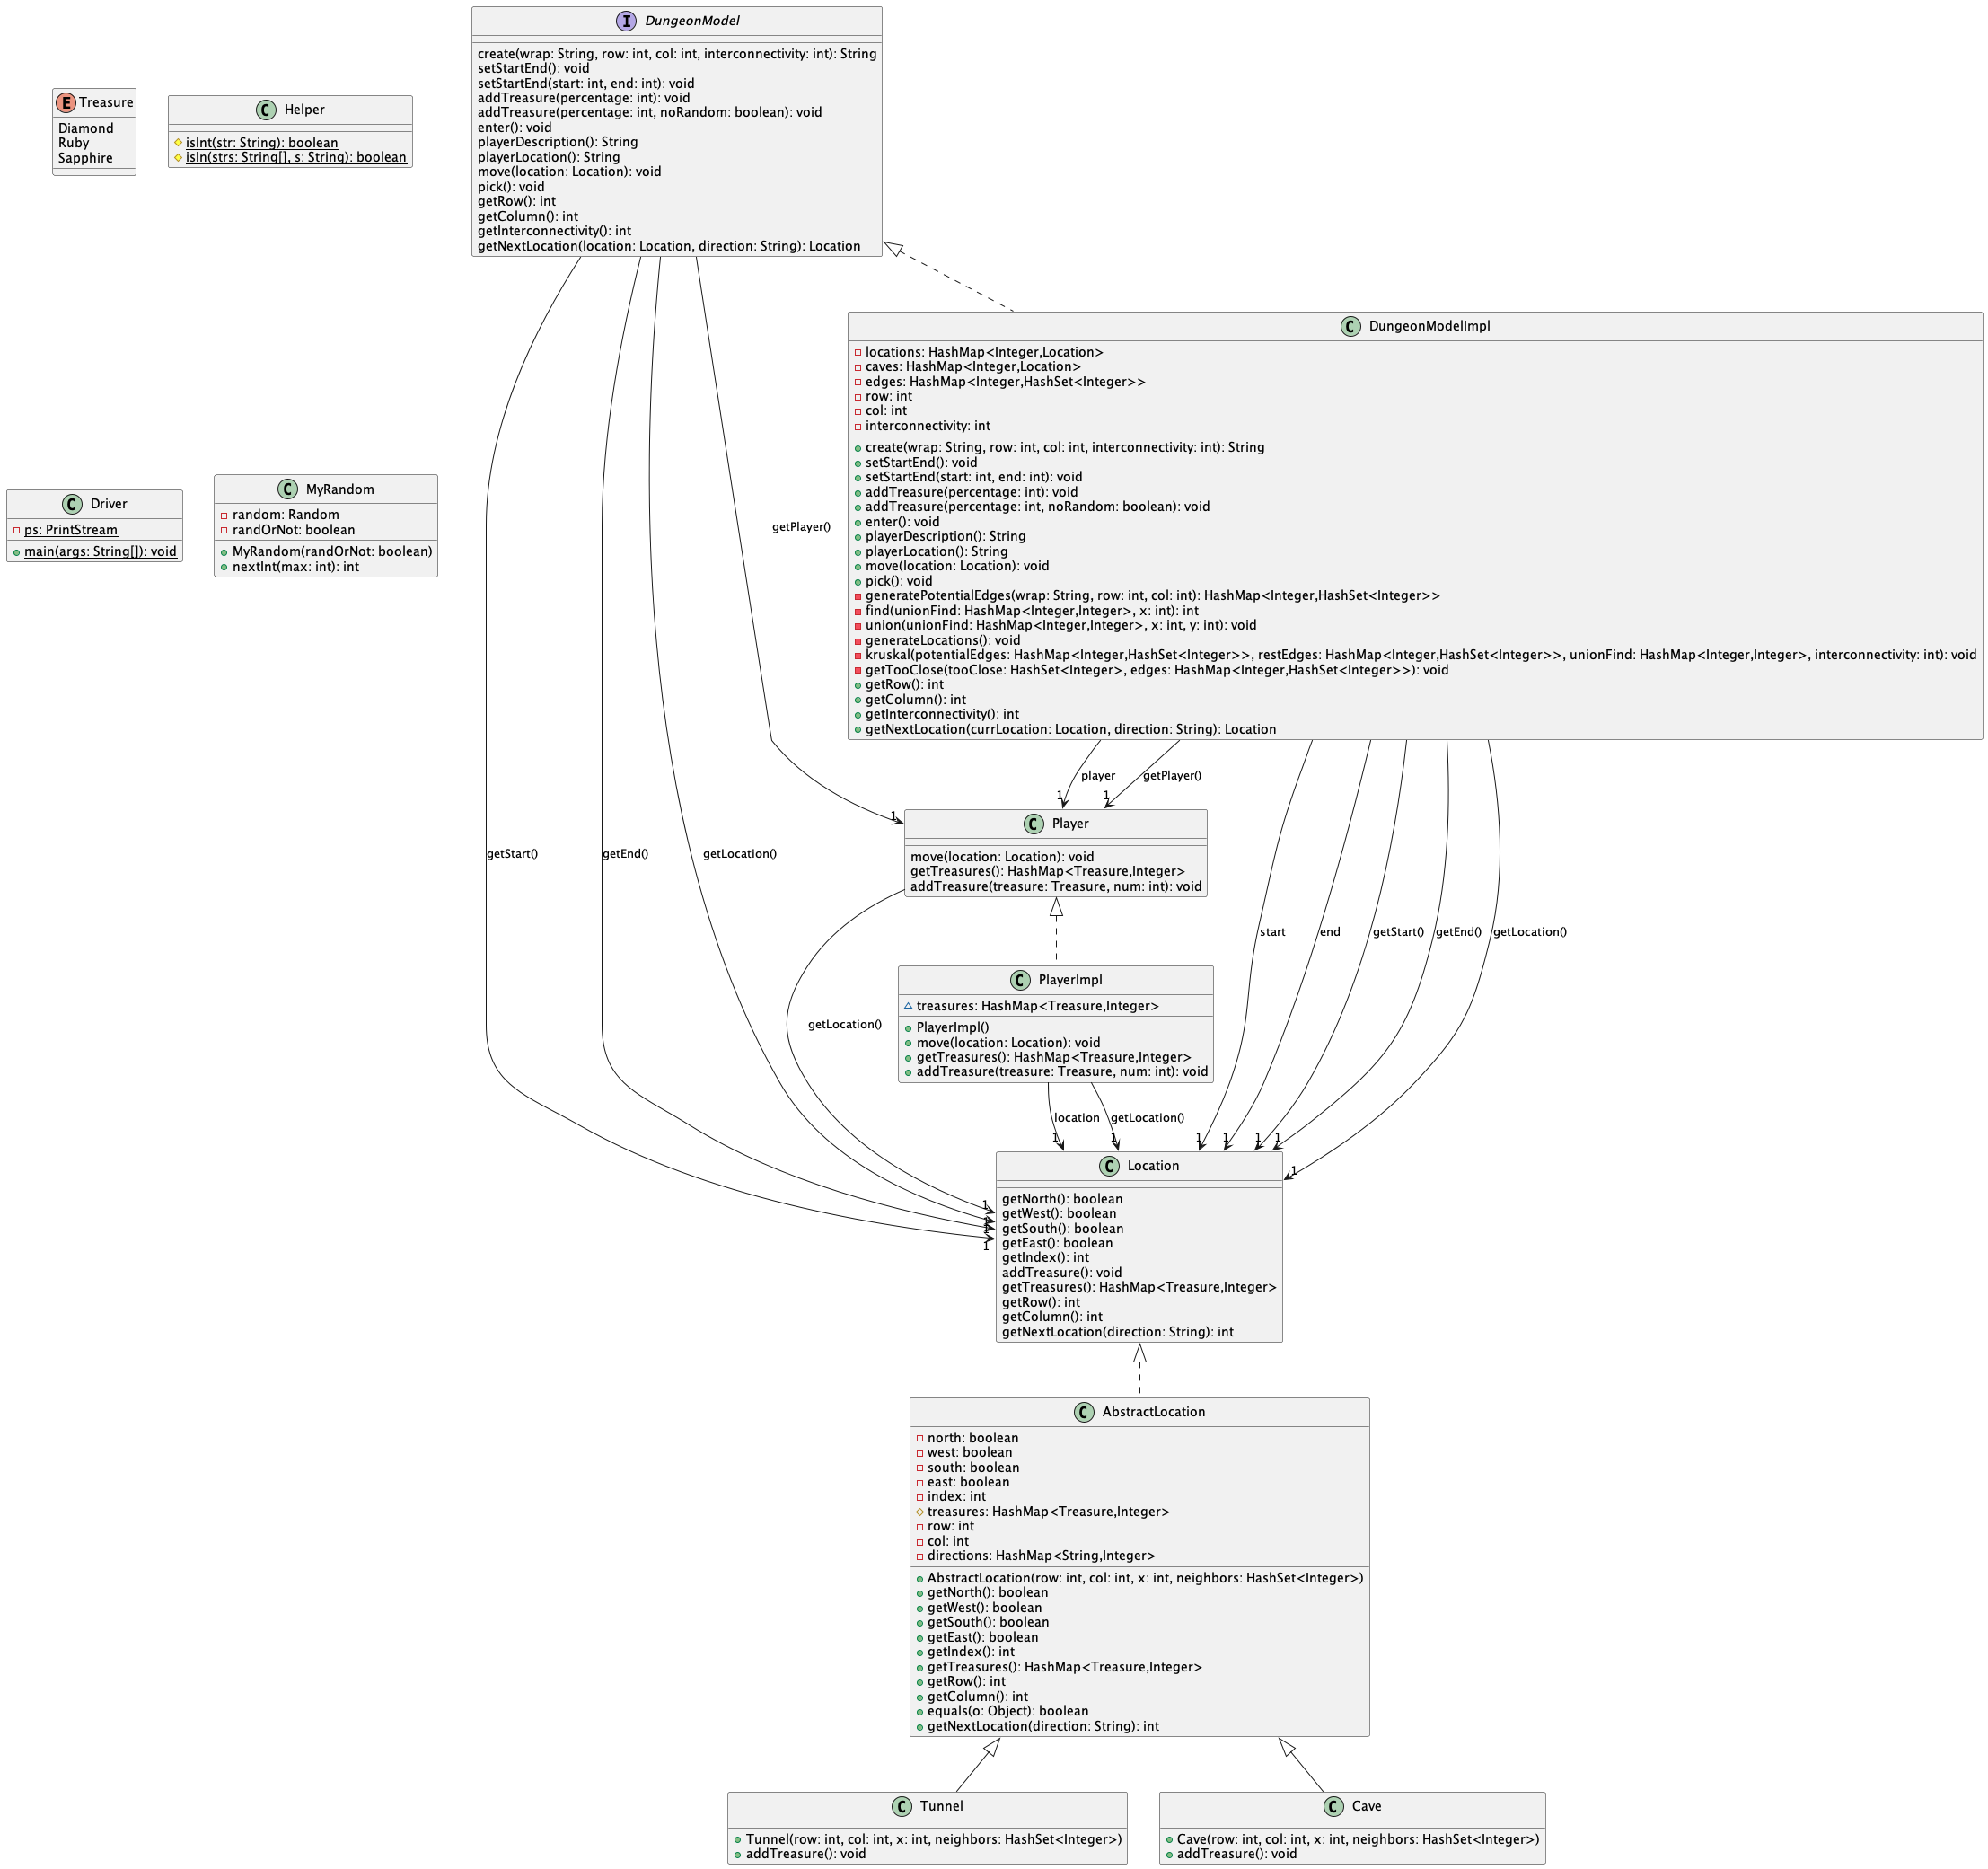
\includegraphics[width=1.2\textwidth]{final_uml.png} %插入图片,[]中设置图片大小,{}中是图片文件名
\end{figure}

\newpage
\section{Test}

\begin{table}[htbp]
   %\topcaption{Table captions are better up top} % requires the topcapt package
   \begin{tabular}{@{} lll @{}} % Column formatting, @{} suppresses leading/trailing space

      Method     & Input & Expected \\
         Constructor   & wrapping constructor    &  Success\\
         Constructor   & non-wrapping constructor     & Success\\
         setStartEnd & Given start and end & Set to the given value\\
         reach all caves & Player traverse the dungeon & Reached all caves\\
         length between start and end & Distance between them & Match\\
         addTreasures & Fixed percent & Required amount of treasures are added\\
         starts at start & The given start location & Match the start location\\
         ends at end & The given end location & Match the final location\\
         playerDescription & A given description & Match the given description\\
         playerLocation & A given description & Match the given description\\
         move & Move to four direction & Successfully changed location\\
         pick & Pick up treasure at current location & Successfully picked treasure\\
         
 
    \end{tabular}
\end{table}

\end{document}